% 第 13 章 Using the PG Pattern Viewer
\bichapter{使用 PG Pattern 查看器}{Using the PG Pattern Viewer}
\label{chap:gui-pg}

IC Compiler II GUI 提供 PG Pattern 窗口，用于创建并预览电源地图案（PG pattern）。用该窗口查看一组预置的 PG pattern 模板（template）。为某个 PG pattern 选定模板之后，把图案模板复制到 PG Pattern Editor，并编辑图案，使之符合设计要求。若图案使用参数（parameter），可以在 PG Pattern 窗口中设置参数。预览图案，并对 Tcl 命令做必要的修改。只有在图案定稿之后，才回到版图窗口，把图案实例化到设计中。

关于 PG Pattern 窗口的更多信息，见下列主题：
\begin{itemize}
  \item 选择 PG Pattern 模板
  \item 预览模板 PG Pattern
  \item 预览已有的图案与策略定义
  \item 高亮单个图案
\end{itemize}

PG Pattern 窗口见图~\ref{fig:gui-147}。

\begin{figure}[htbp]
\centering
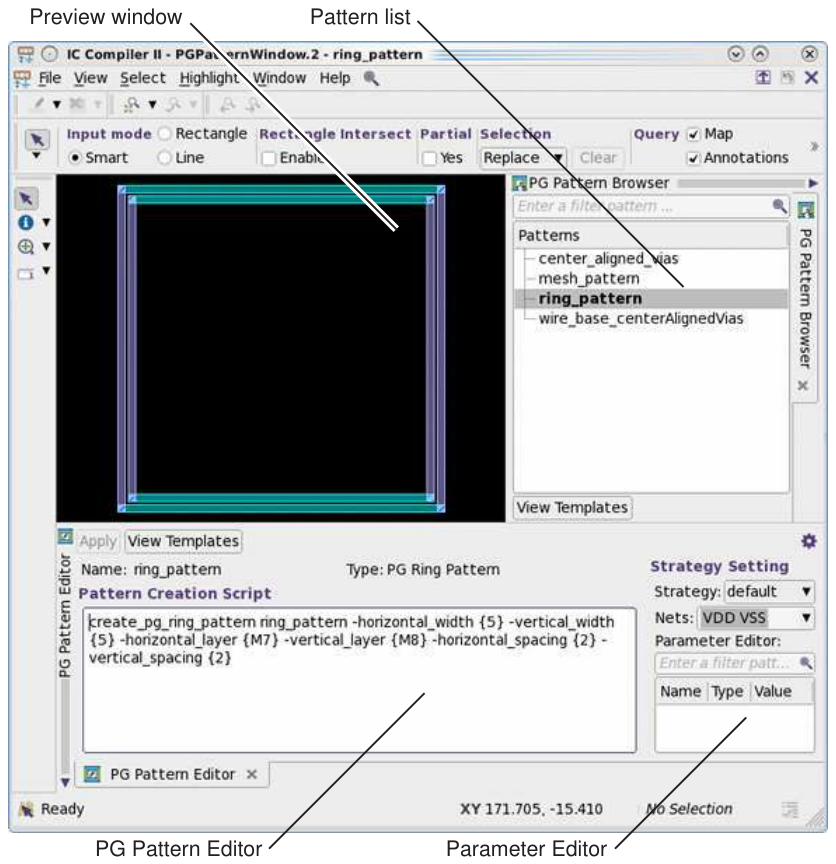
\includegraphics[width=0.92\textwidth]{gui-fig-147.png}
\caption{PG Pattern 窗口}
\label{fig:gui-147}
\end{figure}

图中引出线标出：预览窗口（Preview window）、图案列表（Pattern list）、PG Pattern Editor、Parameter Editor。

\section{选择 PG Pattern 模板}
\subsection*{Selecting a PG Pattern Template}

PG Pattern 窗口包含一组预置模板，可作为创建自己图案的起点。从菜单选择 \textbf{Window > PG Pattern Window}，打开 PG Pattern 窗口。要在 PG Pattern 窗口中查看并选择模板：
\begin{enumerate}
  \item 在 PG Pattern 窗口中单击 View Templates 按钮，打开 PG templates 对话框。
  \item （可选）在 PG Pattern Templates 对话框的过滤模式框中输入字符串，以过滤模板列表。匹配不区分大小写。例如，输入“Mesh”或“mesh”，只显示名称中包含单词 Mesh 的模板。
  \item 在列表中单击模板名以选择模板。工具在 PG Pattern Template 窗口中显示该模板。典型模板包含简短说明、图案图像，以及用于创建该图案的 Tcl 命令。
  \item 单击 Send to Editor 按钮，把模板复制到 PG Pattern 窗口中的 PG Pattern Editor。
\end{enumerate}

\begin{figure}[htbp]
\centering
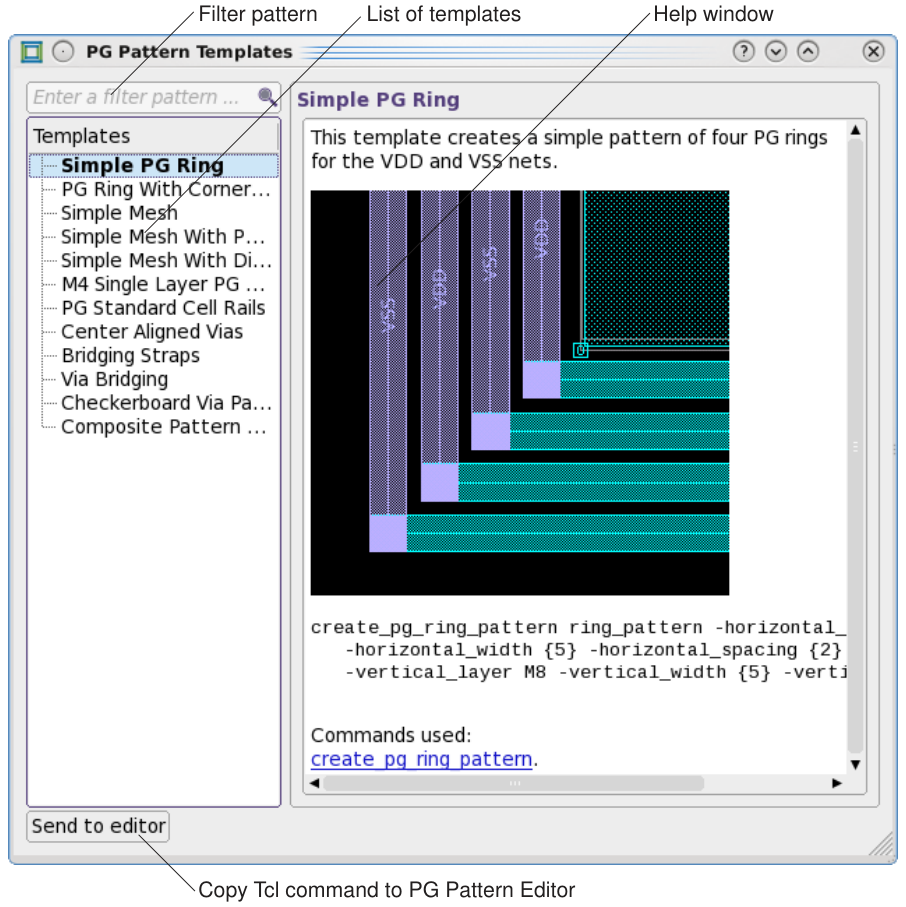
\includegraphics[width=0.92\textwidth]{gui-fig-148.png}
\caption{PG Pattern 模板}
\label{fig:gui-148}
\end{figure}

图中引出线标出：过滤模式（Filter pattern）、模板列表（List of templates）、帮助窗口（Help window），以及把 Tcl 命令复制到 PG Pattern Editor（Copy Tcl command to PG Pattern Editor）。

\section{预览模板 PG Pattern}
\subsection*{Previewing a Template PG Pattern}

图案预览功能在预览窗口中显示模板图案。使用图案预览功能：
\begin{enumerate}
  \item 按“选择 PG Pattern 模板”中所述，把图案模板复制到 PG Pattern Editor。
  \item （可选）修改图案的层、间距、宽度及其他参数，使之与当前设计一致。
  \item 单击 Apply 按钮，在预览窗口中显示图案。
\end{enumerate}

工具会运行 PG Pattern Editor 面板中指定的 \cmd{create\_*\_pattern} 命令，并把图案名加入 PG Pattern Browser 的图案列表。在版图窗口中使用 \cmd{report\_pg\_patterns} 命令，可为设计中当前已定义的图案写出详细报告。创建图案时若出现错误，工具把错误信息写到控制台（console）。

\section{预览已有的图案与策略定义}
\subsection*{Previewing Existing Pattern and Strategy Definitions}

可以用 PG Pattern 窗口按下列步骤预览先前定义的图案和策略：
\begin{enumerate}
  \item 在版图窗口中运行 \cmd{create\_pg\_ring\_pattern}、\cmd{create\_pg\_ring\_pattern} 或其他创建图案的命令，以创建 PG pattern。可以在打开 PG Pattern 窗口之前或之后创建图案。在版图窗口中定义的任何 PG pattern，都会列在 PG Pattern Browser 下的 Patterns 列表中。本例定义了四个环形图案（ring pattern）。

\begin{figure}[htbp]
\centering
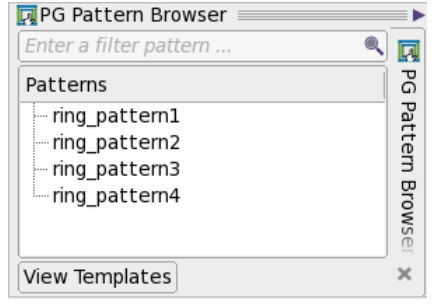
\includegraphics[width=0.92\textwidth]{gui-fig-149.png}
\caption{预定义图案}
\label{fig:gui-149}
\end{figure}

  \item （可选）单击鼠标右键，并从上下文菜单中选择 Delete，以从列表中删除某个图案。

\begin{figure}[htbp]
\centering
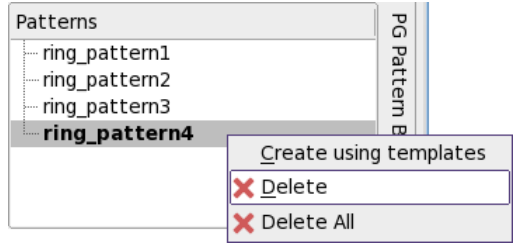
\includegraphics[width=0.92\textwidth]{gui-fig-150.png}
\caption{图案列表的上下文菜单}
\label{fig:gui-150}
\end{figure}

  \item 在列表中单击某个图案以选中它，并在 Pattern Creation Script 编辑器中显示对应的 \cmd{create\_*\_pattern} 命令。
  \item （可选）在编辑器中修改图案。
  \item （可选）用 \cmd{set\_pg\_strategy} 命令创建一个或多个 PG 策略（PG strategy）。
  \item （可选）在 Strategy Setting 下的 Strategy 框中，选择用于创建图案的策略。Strategy 框中只显示所选图案可用的策略。工具也会为所选图案创建一个默认策略。
  \item 单击 Apply，按所选策略和图案在预览窗口中创建图案。

\begin{noteBox}
图案只创建在预览窗口中，不会创建到当前设计的版图窗口里。
\end{noteBox}

  \item （可选）从图案列表中另选一个图案，或从策略框中另选一个策略，并重复上一步，以生成新图案。
\end{enumerate}

\section{高亮单个图案}
\subsection*{Highlighting Individual Patterns}

PG Pattern 查看器支持在一个图案内部高亮各个子图案（child pattern）。用该功能高亮某个图案定义里子图案的电源条带（power strap）和通孔（via），并调整金属层（metal layer）、层宽、间距等。要查看图案中的单个子图案：
\begin{enumerate}
  \item 从图案模板列表中选择图案，例如通孔桥接图案（via bridging pattern）。
  \item 单击鼠标右键，并从列表中选择子图案编号。工具会高亮组成该图案编号的金属形状。
\end{enumerate}

下图为示例 via bridging 复合图案（composite pattern），其中第二个图案被高亮。

\begin{figure}[htbp]
\centering
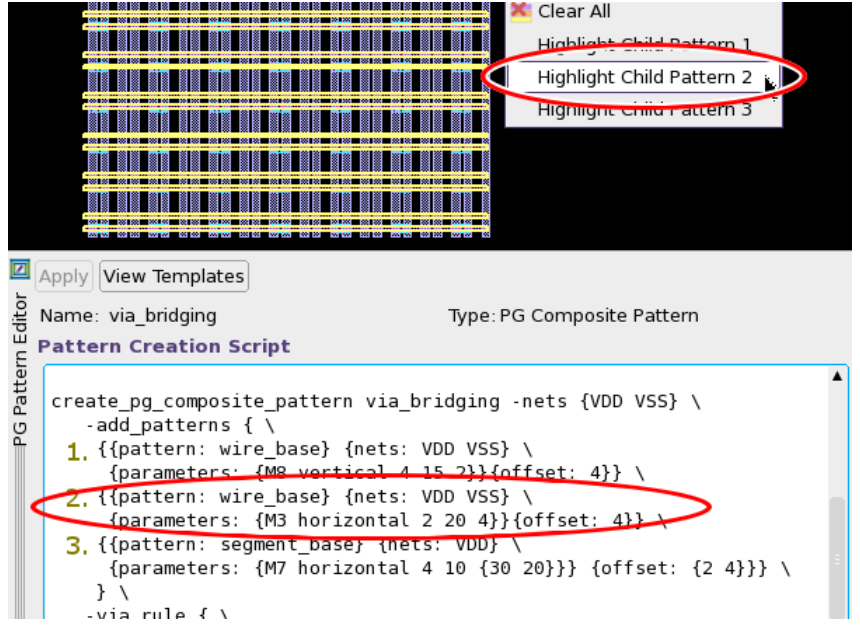
\includegraphics[width=0.92\textwidth]{gui-fig-151.png}
\caption{高亮子图案}
\label{fig:gui-151}
\end{figure}
